% Alternative composition, same constructed inputs and 152.4 mm width.
% Required packages and working directory are the same as ../tikz.tex.
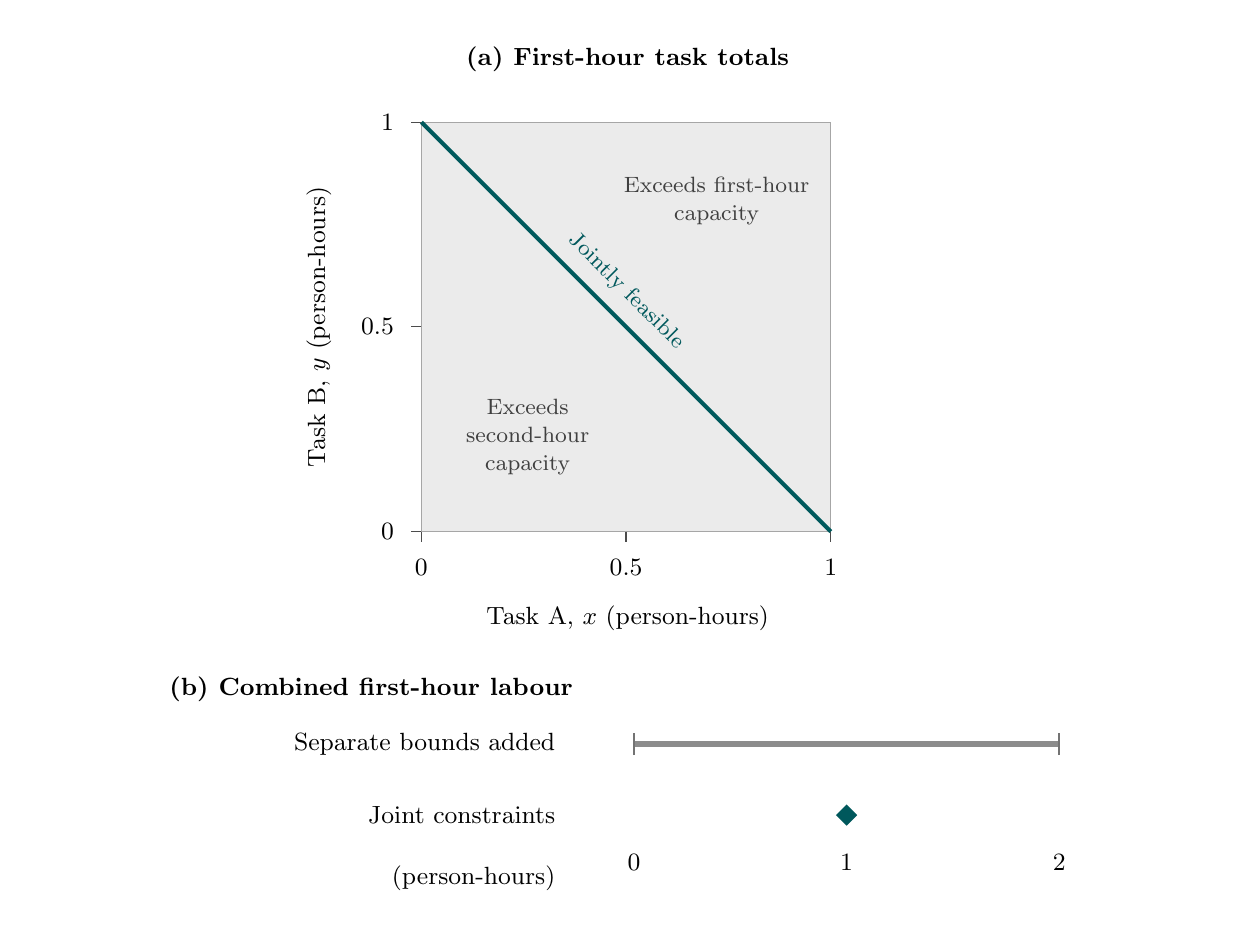
\begin{tikzpicture}[x=1mm,y=1mm,font=\fontsize{9}{11}\selectfont,
  every node/.style={inner sep=0pt,outer sep=0pt}]
  \definecolor{scaccent}{RGB}{0,88,92}
  % Generated by calculate.py; exact derived values, no graphical styling.
\def\SCMarginalMinimum{0}
\def\SCMarginalMaximum{1}
\def\SCTargetBoundary{1}
\def\SCObservationEnd{2}
\def\SCTaskTotal{1}
\def\SCSeparateTotalMinimum{0}
\def\SCSeparateTotalMaximum{2}
\def\SCJointTotal{1}
\def\SCFeasibleStart{(0,1)}
\def\SCFeasibleEnd{(1,0)}
\def\SCFeasibleMidpoint{(0.5,0.5)}
\def\SCTimelineX{0.5}
\def\SCTimelineY{0.5}
\def\SCTaskABlocks{0/0.5,1/1.5}
\def\SCTaskBBlocks{0.5/1,1.5/2}

  \path[use as bounding box] (0,0) rectangle (152.4,111);
  \node[font=\fontsize{9.5}{11.5}\selectfont\bfseries] at (76.2,107)
    {(a) First-hour task totals};
  \begin{scope}[shift={(50,47)},x=52mm,y=52mm]
    \fill[black!8] (0,0) rectangle (1,1);
    \draw[black!35,line width=0.45pt] (0,0) rectangle (1,1);
    \draw[scaccent,line width=1.5pt] \SCFeasibleStart -- \SCFeasibleEnd;
  \end{scope}
  \foreach \v in {0,0.5,1} {
    \draw[black!70,line width=0.45pt] ({50+52*\v},47) -- ({50+52*\v},45.7);
    \node[anchor=north] at ({50+52*\v},43.5) {\v};
    \draw[black!70,line width=0.45pt] (50,{47+52*\v}) -- (48.7,{47+52*\v});
    \node[anchor=east] at (46.5,{47+52*\v}) {\v};
  }
  \node at (76.2,36) {Task A, $x$ (person-hours)};
  \node[rotate=90] at (37,73) {Task B, $y$ (person-hours)};
  \node[align=center,text width=27mm,text=black!75,font=\fontsize{8.5}{10}\selectfont]
    at (87.5,89) {Exceeds first-hour\\capacity};
  \node[align=center,text width=27mm,text=black!75,font=\fontsize{8.5}{10}\selectfont]
    at (63.5,59) {Exceeds second-hour\\capacity};
  \node[rotate=-45,text=scaccent,font=\fontsize{8.5}{10}\selectfont]
    at (76,77.5) {Jointly feasible};
  \node[anchor=west,font=\fontsize{9.5}{11.5}\selectfont\bfseries] at (18,27)
    {(b) Combined first-hour labour};
  \node[anchor=east] at (67,20) {Separate bounds added};
  \node[anchor=east] at (67,11) {Joint constraints};
  \draw[black!45,line width=2pt] (77,20) -- (131,20);
  \foreach \v in {0,2}
    \draw[black!55,line width=0.65pt] ({77+27*\v},18.6) -- ({77+27*\v},21.4);
  \path[fill=scaccent] (104,12.35) -- (105.35,11) -- (104,9.65) -- (102.65,11) -- cycle;
  \foreach \v in {0,1,2} \node at ({77+27*\v},5) {\v};
  \node[anchor=east] at (67,3) {(person-hours)};
\end{tikzpicture}%
